\chapter{Conception}


\section{Planification}

La planification du projet est présentée en détails plus bas. Concernant la gestion interne des taches et de leur avancement, nous utilisons Trello comme requis par l'enseignant responsable de l'UE, en voici le lien d'invitation : \\ \url{https://trello.com/invite/b/HUauMOnv/41ec23e7edb8b51517df475551b7f823/ia-reinforcement-learning}


\begin{center}
\begin{tabularx}{\linewidth}{|p{1cm}|X|p{2.1cm}|p{1cm}|}
    \hline
    ID & Tâche & Antécédents & Durée \\
    \hline
    \hline
    A & Étude de recherche de trésor 1D avec Q-Table & / & 2h \\
    \hline
    B & Programmation de l'IA recherche de trésor 2D avec Q-Table& A & 2h \\
    \hline
    C & Étude du Deep Reinforcement Learning & B & 6h \\
    \hline
    D & Développement d’un environnement générique pour la recherche de trésor & A & 2h \\
    \hline
    E & Développement d’un agent DQN & C & 4h \\
    \hline
    F & Création d’une interface basique & / & 1h \\
    \hline
    G & Création d’une interface avancée & F & 4h \\
    \hline
    H & Développement du système de sauvegarde/chargement d’IA & E & 4h \\
    \hline
    I & Développement du mode ``joueur'' & / & 2h \\
    \hline
    J & Développement d’un agent double DQN & E & 6h \\
    \hline
    K & Développement des tests de l’IA & E & 4h \\
    \hline
    L & Développement d’un agent Q-learning & A & 2h \\
    \hline
    M & Développement du visionnage de l’IA en temps réel & F,L & 2h \\
    \hline
    N & Développement d’agents  RL bonus (si il nous reste du temps après avoir terminé toutes les tâches ci-dessus) & D, G, H, I, J, K, M & 8h \\
    \hline
\end{tabularx}
\end{center}

\begin{figure}
\centering
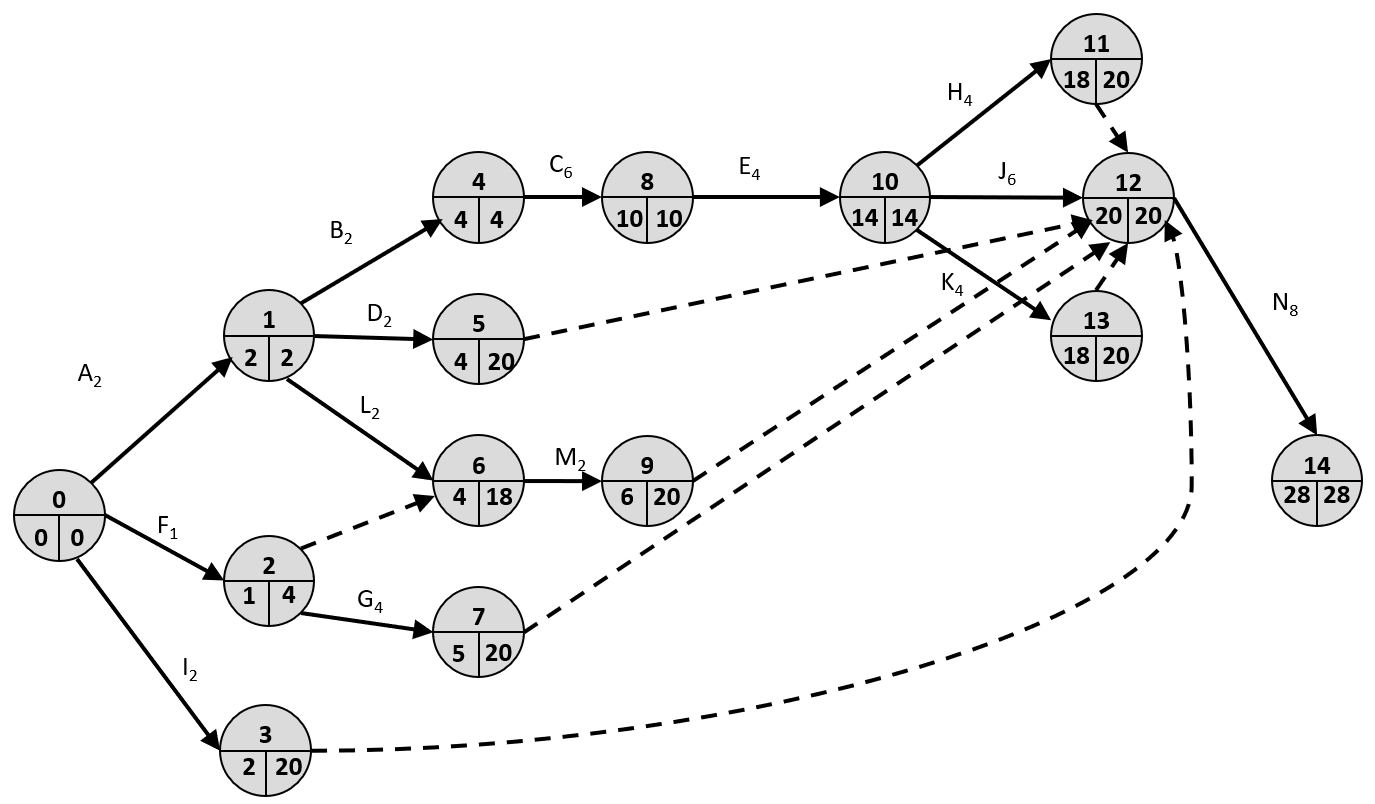
\includegraphics[width=1\textwidth]{pert.png}
\caption{Diagramme de PERT du projet}
\end{figure}

\begin{figure}
\centering
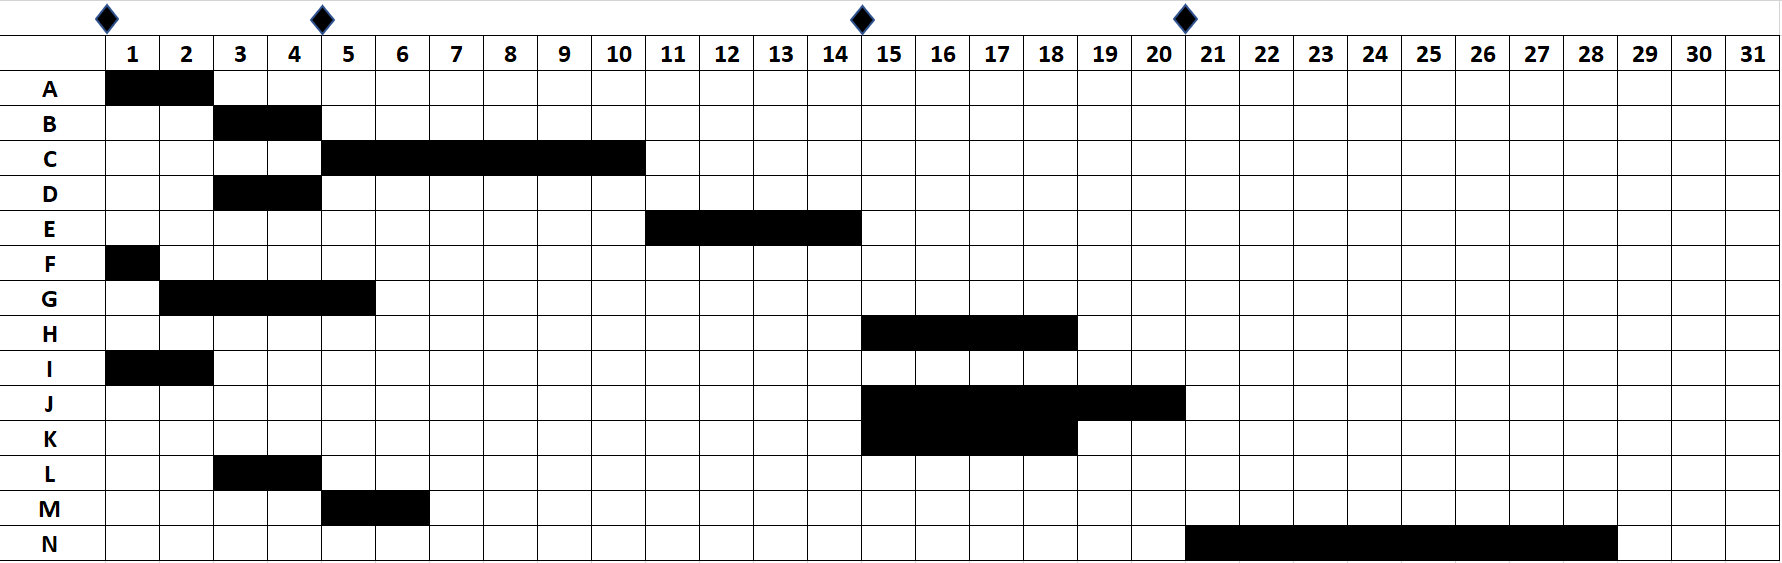
\includegraphics[width=1\textwidth]{gantt.png}
\caption{Diagramme de Gantt original du projet}
\end{figure}

\begin{figure}
\centering
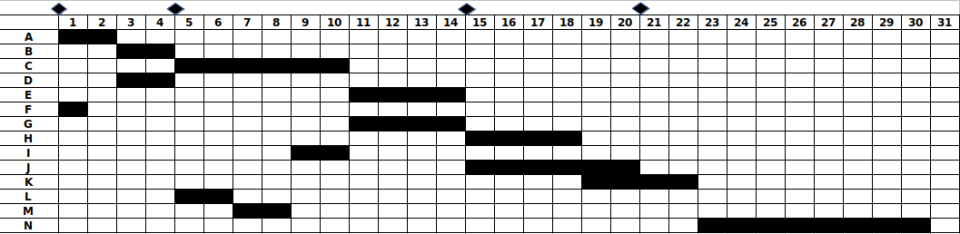
\includegraphics[width=1\textwidth]{gantt_2p.png}
\caption{Diagramme de Gantt adapté à deux personnes}
\end{figure}

L'étape de planification est probablement l'étape du projet la plus complexe à effectuer correctement, c'est donc sans surprise que la planification originalement prévue n'a pas du tout correspondu à la réalité.
\par
La durée estimée de la plupart des tâches était totalement incorrecte, en majorité parce que nous sous-estimions la durée des tâches à effectuer. Le diagramme était pensé pour correspondre au nombre d'heures allouées à l'UE, mais il est en réalité totalement impensable de réussir à terminer ce projet en ne travaillant dessus que 4 heures par semaine.
\par
Le premier objectif du projet fut accompli très rapidement, plus tôt que ce que le diagramme de Gantt prévoyait. Mais le second objectif se révéla être bien plus complexe que prévu, et demanda un grand nombre d'heures de test, de recherche et d'entraînement.
\par
Vous trouverez néanmoins dans cette partie l'ensemble des diagrammes planifiant le déroulement du projet.

\FloatBarrier

\section{Réalisation de la première partie}

La première partie du projet est la réalisation d'un agent capable de jouer (et résoudre, si possible) à la recherche de trésor.

\subsection{Résumé du déroulement}
Bien que la tâche soit relativement simple, au moment où nous commencions le projet, nous ne disposions d'aucune expérience préalable dans le domaine de l'apprentissage par renforcement. Il nous a donc dû fallu nous instruire sur le sujet à l'aide de différentes ressources : cours, articles et exemples.
\par
Notre professeur référent Mme Li nous a redirigé vers son cours sur l'apprentissage par renforcement qu'elle dispense en master, et qui contient une introduction à l'intelligence artificielle, dont l'apprentissage par renforcement à l'aide de Q-Learning \cite{li_rl}. Nous avons aussi consulté différents articles introductifs à l'apprentissage par renforcement, et nous sommes appuyé d'un livre introductif sur le sujet pour en savoir plus sur certains points \cite{rl_an_intro}. Enfin, afin d'observer comment sont implémentées ces connaissances en pratique, nous avons cherché différentes implémentations de Q-Learning que nous avons copié, exécuté, et modifié afin de tenter d'en comprendre le fonctionnement et les structures utilisées \cite{morvanzhou}.
\par
Une fois cette phase de recherche effectuée, nous avons commencé à réimplémenter par nous même le Q-Learning sur la recherche de trésor en 1D. Le principe fut assez vite compris, et la seule difficulté rencontrée était l'utilisation de librairie externe pour manipuler plus rapidement la Q-Table. Suite à cet accomplissement, nous avons reporté notre avancement à notre professeur référent qui nous a proposé d'essayer d'appliquer l'algorithme sur une recherche de trésor en 2D. Cette tâche fut elle aussi assez rapidement effectuée et ne posa pas de problème particulier. Nous nous décidâmes donc à commencer la deuxième partie du projet.

\subsection{Détails de la phase d'implémentation}
Une de premières choses que nous avons fait était de copier un programme déjà existant solvant la recherche de trésor en 1D, et d'en comprendre le fonctionnement. Avant même de tenter de le modifier, nous nous sommes heurté à un problème de compréhension sur le fonctionnement de la Q-Table. Nous avons donc consulté les différentes ressources citées precedemment au fil de notre tentative de compréhension du code afin de comprendre ce qui s'y déroulait exactement.
\par
Une fois le principe de Q-Table compris, nous nous sommes attelé à réécrire le programme de façon plus concise à partir de ce que nous avions compris (l'environnement étant extrêmement simple, la majorité du code n'est que l'agent). La seule partie d'ombre sur le programme était l'affectation tirée de l'équation de Bellman, que nous avions du mal à comprendre intuitivement.
\par
Nous avons ensuite enchaîné sur l'application de notre agent sur un environnement en 2D, et par la même occasion le code fut entièrement réécrit afin de rendre le tout plus propre et compréhensible : le programme en 1D étant très fouillis et confus en raison des essais et modifications pour mieux comprendre son fonctionnement. Cette réécriture fut aussi l'occasion de tester l'orienté objet en Python, qui nous sera utile pour faire des programmes plus conséquents et mieux structurés.
\par
La recherche de trésor en 2D ne posa pas de problème particuliers et ce fut l'occasion de vérifier que nous comprenions bien le fonctionnement d'un agent utilisant le Q-Learning. Seul un point restait quelque peu abstrait : les valeurs des hyperparamètres. Jusqu'ici, nous n'avions pas eu besoin d'y toucher, leur valeurs étaient fixées à $\alpha=0.1$ et $\gamma=0.9$. Bien que nous connaissions leur ``sens'' théorique, notre faible expérience nous empêchait de bien concevoir leur conséquence sur l'apprentissage.

\section{Réalisation de la seconde partie}
La seconde partie du projet est celle ayant posé le plus de problèmes et nous ayant pris le plus de temps. Elle consiste à utiliser le Deep Q-Learning afin de développer un agent capable de jouer à Pac-Man.

\subsection{Choix de l'environnement}
Il est important de noter que OpenAI Gym propose deux versions de chaque jeu Atari où l'état observé par l'agent diffère : dans la première version (nommée \textit{nomjeu-v0}) l'agent observe l'écran du jeu, tandis que dans la deuxième version l'agent observe la RAM du jeu (les jeux Atari 2600 possèdent 128 octets de RAM).
\par
Initialement, nous avions envisagé d'utiliser l'environnement fournissant l'image, puisque cette approche semblait plus ludique et intuitive, toutefois elle requiert quelques connaissances de plus. Nous avons finalement décidé de d'abord ``résoudre'' l'environnement RAM, et si nous avions du temps restant, de résoudre l'environnement avec image.

\subsection{Prémices de la création de l'agent DQN}
L'environnement n'étant pas à notre charge, nous avons directement entamé des recherches pour comprendre le principe du Deep Q-Learning. Bien que son résumé soit simple : ``un réseau de neurone approxime la fonction Q'', cette nouvelle approche apporte son lot de questions et de nouvelles connaissances.
\par
Il nous a d'abord fallu nous mettre à niveau au sujet des réseaux de neurones que nous n'avions alors pas encore abordé lors de notre cursus universitaire \cite{dl_mit, 3b1b_nn, colah}. Dans le même temps, nous tentions de comprendre comment fonctionnait le Deep Q-Learning. Une des difficultés est de réussir à comprendre quels éléments sont des composants essentiels, et quels composants sont des améliorations créées pour rendre le DQN plus efficace. Il est en effet très commun de trouver des implémentations d'agents Double DQN dans des tutoriels, mais commencer par essayer de comprendre une version améliorée du principe rend la tâche plus complexe. Nous avons malgré tout réussi à saisir le fonctionnement du Deep Q-Learning grâce à quelques cours, articles et implémentations \cite{stanford_drl, atari_drl, keon}.

\subsection{Implémentation et premiers tests}
Comme pour la première partie, programmer l'agent fut assez rapide. L'essentiel de la difficulté se trouvant dans le principe, le code n'est pas spécialement long. Une fois implémenté, et pour en tester le bon fonctionnement, nous avons décidé de tester l'agent sur l'environnement de recherche de trésor 2D avec obstacles.
\par
Nous avons été confrontés à notre premier problème de définition de structure du réseau : combien de couches le réseau a-t-il besoin ? Combien de neurones chaque couche doit-elle avoir ?
Nous avons dans un premier temps effectués quelques essais à l'aveugle, avec pour seule connaissance utile que deux couches cachées suffisent à représenter n'importe quelle fonction. Nous supposions que par exemple, dans un environnement à 100 états possibles, un réseau de deux couches cachées de 10 neurones pourrait fonctionner. Mais après quelques essais aléatoires infructueux nous avons décidé de rechercher comment choisir l'architecture d'un réseau selon le problème.
\par
A notre grande surprise, nous avons trouvé qu'il n'existait aucune méthode fiable pour choisir ces paramètres du réseau, c'est majoritairement à l'expérience que la plupart des gens estiment grossièrement l'architecture que le problème requiert. Pour obtenir des architectures optimales il est nécessaire d'utiliser des méthodes capables de faire évoluer l'architecture, il nous est cependant impossible d'en arriver à utiliser de telles méthodes.
\par
Après d'autres essais infructueux, nous commencions à penser que le problème venait sûrement du type d'environnement. En effet, la recherche de trésor est particulièrement basé sur la mémorisation, et surtout sa seule récompense est obtenue en arrivant sur la dernière case. Ce qui veut dire que dans un premier temps, l'agent doit trouver au hasard le trésor, ce qui peut prendre un temps extrêmement long (et qui augmente exponentiellement avec la taille de l'espace de jeu). Puis l'agent doit apprendre le chemin qui remonte jusqu'au trésor à partir de cette seule information. 
\par
De plus, et bien que ce n'est que plus tard que nous l'avons compris avec les recherches pour la partie ``principe des algorithmes utilisés'', l'Experience Replay rend l'apprentissage encore plus complexe. En effet, pour que le réseau apprenne à aller jusqu'à la case d'arrivée, il faut d'abord que la transition de récompense non nulle soit présente dans un des minibatch, selon la taille de l'Experience Replay, du minibatch, et de l'environnement, tomber dessus peut s'avérer très rare.
\par
La recherche de trésor telle que nous l'avons implémenté est donc bien un très mauvais exercice pour les agents DQN, le point majeur à changer dans cet environnement est la fonction de récompense qui donne trop peu d'information sur la performance de l'agent (seulement gagné ou perdu).

\subsection{Première application à Pac-Man}
Suite à nos échecs sur la Recherche de trésor, nous avons décidé de tester l'agent DQN sur Pac-Man. Encore une fois, nos essais se sont tous soldés par des échecs : au terme de l'apprentissage, Pac-Man se retrouvait très souvent bloqué dans des coins sans jamais bouger. Nous ne constations aucune tentative de collecter le maximum de points.
\par
Très vite, nous avons repéré un premier problème : le jeu ne possède pas de récompense négative, la fonction de récompense correspond simplement au score gagné à la frame jouée. OpenAI Gym donnant avec ses environnements l'accès à quelques variables supplémentaires, nous avons pu rajouter une récompense négative dans le cas où le Pac-Man perd une vie (ce qui arrive environ une demi seconde après qu'il ait tué un fantôme).
\par
Cette modification n'a malheureusement pas suffit à améliorer le comportement de l'agent. Notons qu'à ce moment, nous avions déjà implémenté un système de décroissance de la valeur d'$\epsilon$, qui permet de transitionner de choix d'action aléatoire vers un choix plus "raisonné". Mais peu importe la vitesse de décroissance choisie, l'agent n'arrivait pas à un résultat convenable. Ici encore nous avons tenté plusieurs approches d'architecture, mais ici aussi nos essais se sont tous soldés par des échecs.
\par
Il faut aussi noter qu'à cause du système d'apprentissage par minibatch à chaque étape de jeu, la vitesse de jeu est extrêmement lente, et il faut laisser tourner le jeu de nombreuses heures avant d'être sûr de la qualité de l'agent.

\subsection{Application à Cartpole}
Incapable de faire fonctionner l'agent sur Pac-Man, et surtout incapable de trouver un exemple d'architecture ayant déjà résolu ce problème (en apprentissage par renforcement, les jeux Atari 2600 sont relativement communs, mais c'est en général la version où l'agent lit l'écran qui est utilisée), nous décidâmes de tester notre agent sur un environnement plus commun et déjà résolu.
\par
Cartpole est un environnement très simple : dans un environnement en deux dimensions, vu de côté et avec la gravité vers le bas, il faut maintenir un baton à la verticale en déplaçant le chariot le soutenant vers la gauche ou vers la droite.

\begin{figure}
    \centering
    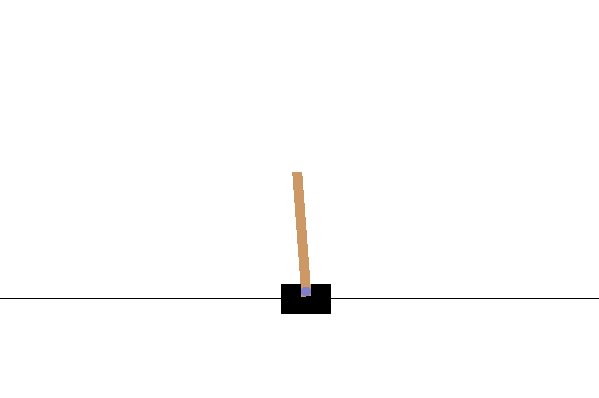
\includegraphics[width=1.0\textwidth]{images/cartpole.png}
    \caption{Représentation graphique de l'environnement CartPole-v1}
    \label{fig:my_label}
\end{figure}

L'environnement observé fournit quatre réels pour décrire son état : la position du chariot, la vitesse du chariot, la rotation du baton et la vitesse de rotation du baton. Les deux actions possibles sont d'accélérer le chariot vers la gauche ou vers la droite. L'objectif est de maintenir le baton à la verticale, l'agent obtient 1 de récompense pour chaque étape de jeu. Le jeu est de durée fixée et ne peut durer plus de 200 étapes. Le jeu est perdu si l'angle du baton par rapport à la verticale est supérieur à 15 degrés.
\par
Cet environnement est extrêmement pratique pour les tests, il est bien connu et on connaît des architectures et hyperparamètres qui fonctionnent. Nous avons donc cherché une solution existante \cite{gsurma_cartpole} et copié ses hyperparamètres et l'architecture de son réseau de neurones.
\par
L'apprentissage a marché sans aucun problème, avec quelques ajustement, nous avons même réussi à obtenir un réseau atteignant un score maximal au bout de 100 épisodes (ce qui arrive très rapidement). Ce test avec CartPole nous a permit de vérifier le bon fonctionnement des algorithmes utilisés par notre agent.
\par
Nous tirons comme conclusion de cette essai que le problème jusqu'ici ne vient pas de notre implémentation d'agent DQN, qui fonctionne parfaitement, mais de nos choix d'hyperparamètres, et de notre architecture de réseau.

\subsection{Application à Breakout}
Pac-Man est un jeu complexe : l'agent doit collecter différents bonus disséminés dans un labyrinthe tout en évitant les ennemis qui le poursuivent. De plus, l'environnement fournit à l'agent toute la RAM de l'Atari 2600 qui contient 128 entiers compris entre 0 et 255 qui devront permettre à l'agent de déduire quelle action il devra effectuer.
\par
Plutôt que de commencer par Pac-Man (duquel on ne connait pas l'architecture optimale, ni les hyperparamètres optimaux), il serait peut-être bénéfiques de réussir à faire résoudre un environnement Atari plus simple à notre agent. Lors de nos recherches nous avons trouvé un exemple de résolution de Breakout ainsi et surtout qu'un papier détaillant la résolution de jeux Atari 2600 en utilisant leur RAM \cite{breakout_tkgw, learn_atari_ram}.
\par
C'est cette dernière ressource qui a joué un rôle capitale dans notre résolution d'environnement Atari. On y trouve en effet de nombreuses améliorations possibles afin d'augmenter l'efficacité de l'agent. L'application de seulement quelques unes de ces dernières permet d'atteindre des performances tout à fait respectables, capables de faire des scores raisonnables sur Breakout.
\par
Nous avons utilisé les valeurs donné à la fin du papier, ainsi que l'architecture ``small ram'' (deux couches cachées de 128 neurones). Ainsi que les hyperparamètres fournis (la majorité d'entre eux proviens d'un autre papier fondateur sur l'application du DQN aux environnements Atari \cite{atari_drl}. Après environ 4 heures d'entraînement, l'agent dépassait régulièrement un score de 20 et continuait de s'améliorer. Les améliorations utilisées sont la normalisation ainsi que le frame skip (définit à 8).
\par
Le Breakout n'étant pas notre objectif, c'est vers Pac-Man que nous avons redirigé nos efforts avec ces nouvelles connaissances.


\subsection{Application à Pac-Man}
\subsubsection{Résumé des améliorations}
Deux de nos problèmes majeurs avec Pac-Man étaient la vitesse de jeu, très lente et qui empêche à l'agent de recueillir un nombre conséquent de situations par le temps qu'il prend à s'entraîner, ainsi que l'impression que le réseau n'arrive pas à apprendre à partir des données fournies.
\par
Le premier problème est réglé par le principe de ``frame skip'', qui consiste simplement à ne fournir à l'agent qu'un instantanné de la RAM sur $n$. Le jeu tourne originalement à 60 images par secondes, à chaque étape l'agent avance d'une image, après 60 étapes il complète une seconde de jeu. Si on prend un frame skip $n=3$, l'agent ne voit qu'une image sur trois, le jeu est pour lui en 20 images par secondes. Cette approche permet d'augmenter drastiquement la vitesse de jeu sans nécessairement y perdre en précision : le jeu est créé pour être joué par un humain ne disposant pas de la capacité d'analyser le jeu 60 fois par secondes. Le seul problème possible peut se présenter si le joueur doit bien ``timer'' ses actions, ce qui n'est pas le cas dans Pac-Man.
\par
Le second problème est réglé par l'utilisation de la normalisation. Cette dernière est très simple : on possède en entrée une liste de 128 octets représentés par des entiers entre 0 et 255, pour les normaliser ont divise simplement l'ensemble de ces entiers par 255. Grâce à cette normalisation, nous nous retrouvons avec une liste de réels compris entre 0 et 1, facilitant ainsi l'apprentissage du réseau de neurones.

\subsubsection{Hyperparamètres et architecture}

Nous réutiliseront les paramètres "classiques" des jeux Atari 2600.

\begin{itemize}
\item learning rate ($\alpha$) = 0.0002
\item discount factor ($\gamma$) = 0.95
\item memory size = $10^6$
\item initial epsilon ($\epsilon$) = 1.0
\item minimal epsilon = 0.05
\item epsilon decay  = 0.997
\item frame skip = 8
\end{itemize}

Notons que $\epsilon$ n'est multiplié par epsilon decay que lorsqu'un épisode est terminé, et non à chaque image de jeu. 
\par
L'architecture de réseau utilisé est calquée sur celle du Breakout : deux couches cachées de 256 neurones chacune (contre 128 pour le breakout, ce choix a été effectué avec l'espoir d'adapter le réseau au nombre d'informations à retenir et prendre en compte dans Pac-Man). La fonction d'activation de ces deux couches est la fonction ReLU, la dernière couche utilise la fonction d'activation identité (ce qui revient au même que n'appliquer aucune fonction).


\subsubsection{Entraînement et analyse des résultats}
Après environ 1000 épisodes d'entraînement, l'agent DQN arrive à dépasser régulièrement un score de 1300. Après 2500 épisodes, nous avons réussi à atteindre un score maximal de 3970.
\par
Nos attentes dans le comportement d'un agent entraîné était que ce dernier apprenne à éviter les fantômes, afin de permettre de survivre le plus longtemps dans le labyrinthe et ainsi augmenter ses chances de compléter le labyrinthe. Cependant, l'agent a trouvé une autre approche bien plus simple et moins subtile : il commence chaque partie par se diriger vers une des quatre super Pac-Gommes, qui permettent à Pac-Man d'être invincible et de manger les fantômes. Il explore ensuite relativement normalement (bien que son exploration soit loin d'être parfaite), en privilégiant l'obtention de super Pac-Gommes. Cette technique, bien que relativement ``bête'' et très éloignée des attentes de techniques d'évitements que nous avions en tête, augmente énormément les chances de faire un score important.


